% !TeX program = lualatex
% ================================================================
% Polish Parallel Text Version of MixedNumberFractionStarters
%
% Generated by the server using the following settings:
%
%   language            Polish (pol)
%   text direction      left to right
%   font                Noto Serif
%   fallback font       Noto Serif
%   built from          latex/starters/targeted/KS3/fractions/mixedNumberFractionStarters.tex
%   vocabulary key      latex/starters/targeted/KS3/fractions/mixedNumberFractionStarters/L2/pol/mixedNumberFractionStarters_polishKey.tex
%   tier 3 vocabulary   green   RGB 0 128 0
%   English text        black   RGB 0 0 0
%   Polish text         purple  RGB 112 48 160
%   layout macros       version 3
%
% Please don't edit any information in this comment block - the server
% compares it against the current settings and rebuilds this file when
% they differ, so changes here would be overwritten. However, feel free
% to make updates to the LaTeX below if you want to edit it.
% ================================================================

\documentclass{beamer}
% ================================================================
% Copied from the English sheet this was translated from, so that
% anything it sets up for itself still works here
% ================================================================
\usepackage{tikz}
\usetikzlibrary{calc}
\usepackage{multicol}
\usepackage{amsmath}
\usepackage{amssymb}

% ================================================================
% Answer-overlay helpers
% ================================================================
\newcommand{\ablank}[1]{%
  \alt<2>{\textcolor{red}{#1}}{\underline{\phantom{#1}}}%
}
\newcommand{\ashow}[1]{\uncover<2->{\textcolor{red}{\small #1}}}
\newcommand{\ashowq}[1]{\alt<2->{\textcolor{red}{\small #1}}{?}}

% Answers drawn straight on to a TikZ diagram, revealed on overlay 2 like \ashow.
% Space is reserved on overlay 1, so the diagram does not move between slides.
\usetikzlibrary{overlay-beamer-styles}
\tikzset{
  ans/.style     = {red, thick, visible on=<2->},
  ansfill/.style = {red!15, visible on=<2->},
  anslab/.style  = {red, font=\tiny, visible on=<2->},
}

\title{Fractions: Adding \& Subtracting}
\author{}
\date{}

% Characters this language's font has not got are borrowed from another,
% rather than being silently dropped - see docs/translated-sheet-latex.md
\directlua{%
  if luaotfload and luaotfload.add_fallback then
    luaotfload.add_fallback("eallatinfallback",
      { "Noto Serif:mode=harf;" })
  else
    tex.error("this luaotfload is too old to register a fallback font")
  end
}
\usepackage[english]{babel}
\babelprovide[import]{polish}
\babelfont[polish]{rm}[Renderer=Harfbuzz, BoldFont={Noto Serif}, ItalicFont={Noto Serif}, BoldItalicFont={Noto Serif}, RawFeature={fallback=eallatinfallback}]{Noto Serif}
\babelfont[polish]{sf}[Renderer=Harfbuzz, BoldFont={Noto Serif}, ItalicFont={Noto Serif}, BoldItalicFont={Noto Serif}, RawFeature={fallback=eallatinfallback}]{Noto Serif}
\newcommand{\ealtext}[1]{\foreignlanguage{polish}{#1}}
\newcommand{\ealtextblock}[1]{{\raggedright\foreignlanguage{polish}{#1}\par}}
% ================================================================
% EAL layout helpers
% ================================================================
\usepackage{xcolor}

\definecolor{ealkeycolour}{RGB}{0,128,0}
\definecolor{ealenglish}{RGB}{0,0,0}
\definecolor{ealtwocolour}{RGB}{112,48,160}

\newsavebox{\ealboxen}
\newsavebox{\ealboxtr}
\newlength{\ealglosswd}
\newlength{\ealglossraise}
\setlength{\ealglossraise}{1.15em}

% a tier 3 word, in English and in translation alike
\newcommand{\ealkey}[1]{\textcolor{ealkeycolour}{#1}}
\newcommand{\ealkeytr}[1]{\textcolor{ealkeycolour}{\ealtext{#1}}}

% One translated word above one English word. Built from kernel
% primitives, never a tabular, which would break wherever the sheet
% loads array, booktabs or tabularx. The box is as wide as the wider of
% the two, so a long translation pushes its neighbours aside instead of
% overlapping them, and it claims its full height so a table row or a
% TikZ node makes room for it.
\newcommand{\ealgloss}[2]{%
  \sbox{\ealboxen}{\ealkey{#1}}%
  \sbox{\ealboxtr}{\small\textcolor{ealtwocolour}{\ealtext{#2}}}%
  \setlength{\ealglosswd}{\wd\ealboxen}%
  \ifdim\wd\ealboxtr>\ealglosswd\setlength{\ealglosswd}{\wd\ealboxtr}\fi
  \leavevmode
  \makebox[\ealglosswd][c]{%
    \makebox[0pt][c]{\usebox{\ealboxen}}%
    \makebox[0pt][c]{\raisebox{\ealglossraise}{\usebox{\ealboxtr}}}%
  }%
}

% opens up line spacing around a block of glosses, so the raised
% translations sit clear of the line above
\newenvironment{ealglossed}{\par\linespread{2.1}\selectfont\ignorespaces}{\par}

% a whole translated sentence above its English counterpart. block level,
% so it does not belong inside a tabular cell
\newcommand{\ealpara}[2]{%
  \par\addvspace{0.5\baselineskip}%
  {\color{ealtwocolour}\ealtextblock{#1}}%
  \penalty200
  {\color{ealenglish}#2\par}%
  \addvspace{0.5\baselineskip}%
}

\begin{document}

\frame{\titlepage}

%------------------------------------------------
% SLIDE 10: Introduction to Adding Fractions (Same Denominator)
%------------------------------------------------
\begin{frame}[allowframebreaks]{Starter 10}

\vspace{-2em}

\begin{columns}

\column{0.2\textwidth}
\begin{center}
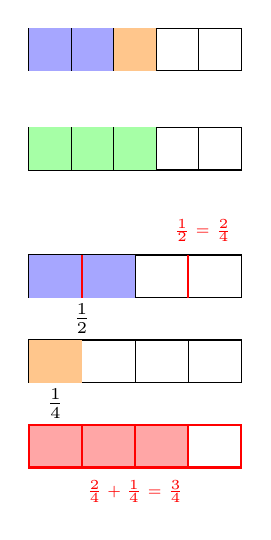
\begin{tikzpicture}[scale=0.9]

\draw (0,1) rectangle (3,1.6);
\fill[blue!35] (0,1) rectangle (1.2,1.6);
\fill[orange!45] (1.2,1) rectangle (1.8,1.6);
\foreach \x in {0.6,1.2,1.8,2.4} \draw (\x,1) -- (\x,1.6);
\draw (0,-0.4) rectangle (3,0.2);
\fill[green!35] (0,-0.4) rectangle (1.8,0.2);
\foreach \x in {0.6,1.2,1.8,2.4} \draw (\x,-0.4) -- (\x,0.2);

\draw (0,-2.2) rectangle (3,-1.6);
\draw (1.5,-2.2) -- (1.5,-1.6);
\fill[blue!35] (0,-2.2) rectangle (1.5,-1.6);
\node at (0.75,-2.5) {\small $\frac{1}{2}$};
\draw (0,-3.4) rectangle (3,-2.8);
\foreach \x in {0.75,1.5,2.25} \draw (\x,-3.4) -- (\x,-2.8);
\fill[orange!45] (0,-3.4) rectangle (0.75,-2.8);
\node at (0.375,-3.7) {\small $\frac{1}{4}$};

% --- Q6 answer: split the half into quarters, then 2/4 + 1/4 = 3/4 ---
\draw[ans] (0.75,-2.2) -- (0.75,-1.6);
\draw[ans] (2.25,-2.2) -- (2.25,-1.6);
\node[anslab, above left] at (3,-1.55) {$\tfrac{1}{2}=\tfrac{2}{4}$};
\fill[ansfill, red!35] (0,-4.6) rectangle (2.25,-4.0);
\draw[ans] (0,-4.6) rectangle (3,-4.0);
\foreach \x in {0.75,1.5,2.25} \draw[ans] (\x,-4.6) -- (\x,-4.0);
\node[anslab, below] at (1.5,-4.65) {$\tfrac{2}{4}+\tfrac{1}{4}=\tfrac{3}{4}$};
\end{tikzpicture}
\end{center}

\column{0.8\textwidth}
\small
\begin{enumerate}
  \item \ealpara{\ealkeytr{Uprość} całkowicie: $\dfrac{12}{16}$}{Fully \ealkey{simplify}: $\dfrac{12}{16}$}
  \ashow{$=\frac{3}{4}$}
  \item \ealpara{Który jest większy: $\dfrac{3}{7}$ czy $\dfrac{3}{9}$?}{Which is larger: $\dfrac{3}{7}$ or $\dfrac{3}{9}$?}
  \ashow{$\frac{3}{7}$}
  \item \ealpara{Przekształć $\dfrac{11}{4}$ na \ealkeytr{liczbę mieszaną}.}{Convert $\dfrac{11}{4}$ to a \ealkey{mixed number}.}
  \ashow{$=2\frac{3}{4}$}
  \item \ealpara{Uzupełnij dodawanie przedstawione na słupkach po lewej:}{Complete the addition represented by the bars to the left:}
  $$\color{blue}\dfrac{\text{{\ashowq{2}}}}{5} \color{orange} + \dfrac{\text{{\ashowq{1}}}}{5} \color{green} = \dfrac{3}{\text{{\ashowq{5}}}}$$
  \item \ealpara{Oblicz:}{Calculate:}
  \[
    \frac{1}{7} + \frac{3}{7} \qquad \frac{5}{9} + \frac{2}{9}
  \]
  \ashow{$=\frac{4}{7},\ \frac{7}{9}$}
  \item \ealpara{Aby dodać $\dfrac{1}{2} + \dfrac{1}{4}$, co musisz najpierw zrobić? Czy możesz narysować obrazek, aby to pokazać?}{To add $\dfrac{1}{2} + \dfrac{1}{4}$, what must you do first? Can you draw a picture to demonstrate?}
  \ashow{Znajdź \ealkeytr{wspólny mianownik}: $\frac12=\frac24$, więc $\frac24+\frac14=\frac34$.}
  \ashow{Find a \ealkey{common denominator}: $\frac12=\frac24$, so $\frac24+\frac14=\frac34$.}
\begin{multicols}{2}
  \item \ealpara{Oblicz: $\dfrac{1}{2} + \dfrac{1}{4}$}{Calculate: $\dfrac{1}{2} + \dfrac{1}{4}$}
  \ashow{$=\frac{3}{4}$}
  \item \ealpara{Oblicz: $\dfrac{1}{3} + \dfrac{1}{4}$}{Calculate: $\dfrac{1}{3} + \dfrac{1}{4}$}
  \ashow{$=\frac{7}{12}$}
\end{multicols}
\end{enumerate}

\end{columns}
\end{frame}


%------------------------------------------------
% SLIDE 11: Subtracting Fractions
%------------------------------------------------
\begin{frame}[allowframebreaks]{Starter 11}

\vspace{-2em}

\begin{columns}

\column{0.2\textwidth}

\begin{center}

\vspace{-5em}
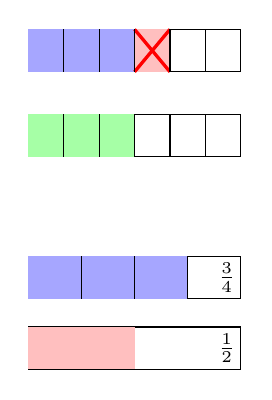
\begin{tikzpicture}[scale=0.9]

\draw (0,4) rectangle (3,4.6);
\fill[blue!35] (0,4) rectangle (2,4.6);
\fill[red!25] (1.5,4) rectangle (2,4.6);
\draw[red, very thick] (1.5,4) -- (2,4.6);
\draw[red, very thick] (2,4) -- (1.5,4.6);
\foreach \x in {0.5,1,1.5,2,2.5} \draw (\x,4) -- (\x,4.6);

\draw (0,2.8) rectangle (3,3.4);
\fill[green!35] (0,2.8) rectangle (1.5,3.4);
\foreach \x in {0.5,1,1.5,2,2.5} \draw (\x,2.8) -- (\x,3.4);

\draw (0,0.8) rectangle (3,1.4);
\fill[blue!35] (0,0.8) rectangle (2.25,1.4);
\foreach \x in {0.75,1.5,2.25} \draw (\x,0.8) -- (\x,1.4);
\node at (2.8,1.1) {\small $\frac{3}{4}$};

\draw (0,-0.2) rectangle (3,0.4);
\draw (1.5,-0.2) -- (1.5,0.4);
\fill[red!25] (0,-0.2) rectangle (1.5,0.4);
\node at (2.8,0.1) {\small $\frac{1}{2}$};

\end{tikzpicture}
\end{center}

\column{0.8\textwidth}
\small
\begin{enumerate}
  \item \ealpara{Zapisz 3 \ealkeytr{ułamki} \ealkeytr{równoważne} $\dfrac{2}{3}$.}{Write 3 \ealkey{fractions} \ealkey{equivalent} to $\dfrac{2}{3}$.}
  \ashow{$\frac46,\frac69,\frac{8}{12}$}
  \item \ealpara{Ustaw od najmniejszej do największej: $\dfrac{1}{8}, \ \dfrac{1}{2}, \ \dfrac{1}{12}$}{Order smallest to largest: $\dfrac{1}{8}, \ \dfrac{1}{2}, \ \dfrac{1}{12}$}
  \ashow{$\frac{1}{12}<\frac{1}{8}<\frac{1}{2}$}
  \item \ealpara{Przekształć $2\dfrac{3}{7}$ na \ealkeytr{ułamek niewłaściwy}.}{Convert $2\dfrac{3}{7}$ to an \ealkey{improper fraction}.}
  \ashow{$=\frac{17}{7}$}
  \item \ealpara{Uzupełnij odejmowanie przedstawione na słupkach po lewej:}{Complete the subtraction represented by the bars to the left:}
  $$\color{blue}\dfrac{4}{6} \color{red}- \dfrac{\text{{\ashowq{1}}}}{6} \color{green} = \dfrac{\text{{\ashowq{3}}}}{6} \color{black} = \dfrac{1}{\text{{\ashowq{2}}}}$$
  \item \ealpara{Oblicz:}{Calculate:}
  \[
    \frac{7}{10} - \frac{3}{10} \qquad \frac{8}{9} - \frac{5}{9}
  \]
  \ashow{$=\frac{2}{5},\ \frac{1}{3}$}
  \item \ealpara{Użyj słupków, aby obliczyć $\dfrac{3}{4} - \dfrac{1}{2}$.}{Use the bars to work out $\dfrac{3}{4} - \dfrac{1}{2}$.}
  \ashow{$=\frac{1}{4}$}
  \begin{multicols}{2}
  \item \ealpara{Oblicz: $\dfrac{5}{6} - \dfrac{1}{4}$}{Calculate: $\dfrac{5}{6} - \dfrac{1}{4}$}
  \ashow{$=\frac{7}{12}$}
  \item \ealpara{Oblicz: $\dfrac{7}{8} - \dfrac{2}{3}$}{Calculate: $\dfrac{7}{8} - \dfrac{2}{3}$}
  \ashow{$=\frac{5}{24}$}
  \end{multicols}
  \vspace{-2em}
  \item \ealpara{Ustaw od najmniejszej do największej: $\dfrac{3}{8},\ \dfrac{1}{2},\ \dfrac{5}{12}$}{Order smallest to largest: $\dfrac{3}{8},\ \dfrac{1}{2},\ \dfrac{5}{12}$}
  \ashow{$\frac{3}{8}<\frac{5}{12}<\frac{1}{2}$}
\end{enumerate}

\end{columns}
\end{frame}


%------------------------------------------------
% SLIDE 12: Mixed Numbers — Adding
%------------------------------------------------
\begin{frame}[allowframebreaks]{Starter 12}

\vspace{-2em}

\begin{columns}

\column{0.3\textwidth}
\vspace{-5em}
\begin{center}
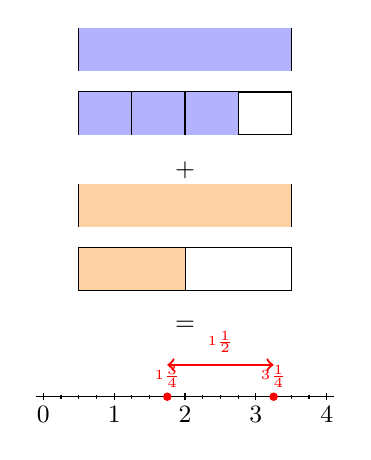
\begin{tikzpicture}[scale=0.9]
% Two wholes side by side as bars (1 3/4 + 1 1/2)
% 1st whole
\draw (0,5) rectangle (3,5.6);
\fill[blue!30] (0,5) rectangle (3,5.6);
% 3/4 part
\draw (0,4.1) rectangle (3,4.7);
\fill[blue!30] (0,4.1) rectangle (2.25,4.7);
\foreach \x in {0.75,1.5,2.25} \draw (\x,4.1) -- (\x,4.7);
\node at (1.5,3.6) {\small $+$};
% 2nd whole
\draw (0,2.8) rectangle (3,3.4);
\fill[orange!35] (0,2.8) rectangle (3,3.4);
% 1/2 part
\draw (0,1.9) rectangle (3,2.5);
\draw (1.5,1.9) -- (1.5,2.5);
\fill[orange!35] (0,1.9) rectangle (1.5,2.5);
\node at (1.5,1.4) {\small $=$};
% Number line
\draw (-0.6,0.4) -- (3.6,0.4);
\foreach \x/\lab in {0/0,1/1,2/2,3/3,4/4} {
  \draw (\x-0.5,0.35) -- (\x-0.5,0.45);
  \node at (\x-0.5,0.15) {\small \lab};
}
\foreach \x in {0,1,2,3} {
  \foreach \q in {0.25,0.5,0.75} {
    \draw (\x+\q-0.5,0.37) -- (\x+\q-0.5,0.43);
  }
}

% --- Q5 answer: the two mixed numbers marked, with the difference between them ---
\fill[ans] (1.25,0.4) circle (0.06);
\node[anslab, above, inner sep=2pt] at (1.25,0.45) {$1\tfrac{3}{4}$};
\fill[ans] (2.75,0.4) circle (0.06);
\node[anslab, above, inner sep=2pt] at (2.75,0.45) {$3\tfrac{1}{4}$};
\draw[ans, <->] (1.25,0.85) -- (2.75,0.85);
\node[anslab, above] at (2,0.88) {$1\tfrac{1}{2}$};
\end{tikzpicture}
\end{center}

\column{0.7\textwidth}
\small
\begin{enumerate}
\begin{multicols}{3}
  \item $\dfrac{2}{5} + \dfrac{1}{5}$ \ashow{$=\frac{3}{5}$}
  \item $\dfrac{3}{4} - \dfrac{1}{2}$ \ashow{$=\frac{1}{4}$}
  \item \ealpara{\ealkeytr{Uprość}: $\dfrac{36}{48}$}{\ealkey{Simplify}: $\dfrac{36}{48}$}
  \ashow{$=\frac{3}{4}$}
\end{multicols}
  
  \item \ealpara{Uzupełnij luki, korzystając z diagramu:}{Fill in the blanks using the diagram:}
  \[
    \color{blue}\text{{\ashowq{1}}}\frac{\text{{\ashowq{3}}}}{4} \color{orange} + 1\frac{\text{{\ashowq{1}}}}{\text{{\ashowq{2}}}} \color{black} = \frac{\text{{\ashowq{7}}}}{4} + \frac{\text{{\ashowq{6}}}}{4} = \frac{\text{{\ashowq{13}}}}{4} = \ \text{{\ashowq{3}}}  \frac{1}{\text{{\ashowq{4}}}}
  \]
  \begin{multicols}{2}
  \item 
  \[
    2\frac{1}{3} + 1\frac{1}{3}
  \]
  \ashow{$=3\frac{2}{3}$}
  \item 
  \[
    3\frac{1}{4} + 1\frac{1}{2}
  \]
  \ashow{$=4\frac{3}{4}$}
  \end{multicols}
  \item \ealpara{Zaznacz $1\dfrac{3}{4}$ i $3\dfrac{1}{4}$ na \ealkeytr{osi liczbowej}. Jaka jest \ealkeytr{różnica}? Jak inaczej możesz to obliczyć?}{Mark $1\dfrac{3}{4}$ and $3\dfrac{1}{4}$ on the \ealkey{number line}. What is the \ealkey{difference}? How else could you work this out?}
  \ashow{Różnica $=\frac{3}{2}=1\frac12$; oblicz jako $3\frac14-1\frac34=\frac{13}{4}-\frac{7}{4}=\frac{6}{4}=\frac{3}{2}$.}
  \ashow{\ealkey{Difference} $=\frac{3}{2}=1\frac12$; work out as $3\frac14-1\frac34=\frac{13}{4}-\frac{7}{4}=\frac{6}{4}=\frac{3}{2}$.}
  \begin{multicols}{2}
  \item \ealpara{Oblicz: $2\dfrac{2}{3} + 1\dfrac{3}{4}$}{Calculate: $2\dfrac{2}{3} + 1\dfrac{3}{4}$}
  \ashow{$=4\frac{5}{12}$}
  \item \ealpara{Oblicz $1\dfrac{3}{4} - 3\dfrac{1}{4} $}{Calculate $1\dfrac{3}{4} - 3\dfrac{1}{4} $}
  \ashow{$=-1\frac{1}{2}$}
  \end{multicols}
\end{enumerate}

\end{columns}
\end{frame}


%------------------------------------------------
% SLIDE 13: Mixed Numbers — Subtracting (improper fraction method)
%------------------------------------------------
\begin{frame}[allowframebreaks]{Starter 13}
\vspace{-2em}
\begin{columns}
\column{0.25\textwidth}

\vspace{-7em}

\begin{center}
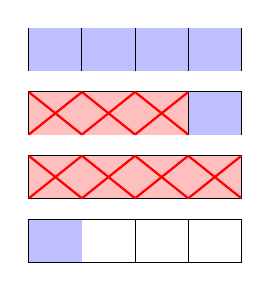
\begin{tikzpicture}[scale=0.9]
% Show 13/4 as bars (3 whole bars + 1/4)
\foreach \y in {3.8,2.9,2.0} {
  \draw (0,\y) rectangle (3,\y+0.6);
  \fill[blue!25] (0,\y) rectangle (3,\y+0.6);
  \foreach \x in {0.75,1.5,2.25} \draw (\x,\y) -- (\x,\y+0.6);
}
\draw (0,1.1) rectangle (3,1.7);
\foreach \x in {0.75,1.5,2.25} \draw (\x,1.1) -- (\x,1.7);
\fill[blue!25] (0,1.1) rectangle (0.75,1.7);

% Cross out 1 3/4 = 7 quarter-segments
% That's all 4 quarters of one whole bar + 3 quarters of another
% Cross out all 4 quarters of the bottom whole bar (y=2.0)
\foreach \i in {0,1,2,3} {
  \fill[red!25] ({0.75*\i},2.0) rectangle ({0.75*\i+0.75},2.6);
  \draw[red, thick] ({0.75*\i},2.0) -- ({0.75*\i+0.75},2.6);
  \draw[red, thick] ({0.75*\i+0.75},2.0) -- ({0.75*\i},2.6);
}
% Cross out 3 quarters of the next bar (y=2.9)
\foreach \i in {0,1,2} {
  \fill[red!25] ({0.75*\i},2.9) rectangle ({0.75*\i+0.75},3.5);
  \draw[red, thick] ({0.75*\i},2.9) -- ({0.75*\i+0.75},3.5);
  \draw[red, thick] ({0.75*\i+0.75},2.9) -- ({0.75*\i},3.5);
}

\end{tikzpicture}
\end{center}

\column{0.75\textwidth}
\small
\begin{enumerate}
  
  \item \ealpara{Która jest większa: $2\dfrac{1}{3}$ czy $2\dfrac{2}{5}$?}{Which is greater: $2\dfrac{1}{3}$ or $2\dfrac{2}{5}$?}
  \ashow{$2\frac{2}{5}$}
  \item \ealpara{Przekształć $\dfrac{23}{6}$ na \ealkeytr{liczbę mieszaną}.}{Convert $\dfrac{23}{6}$ to a \ealkey{mixed number}.}
  \ashow{$=3\frac{5}{6}$}
  \item \ealpara{Rozważ diagram po lewej, uzupełnij luki, aby pokazać odejmowanie za pomocą \ealkeytr{ułamków niewłaściwych}:}{Consider the diagram on the left, fill in the blanks to demonstrate subtraction using \ealkey{improper fractions}:}
  \[
    3\frac{1}{4} - 1\frac{3}{4} = \frac{\text{{\ashowq{13}}}}{4} - \frac{\text{{\ashowq{7}}}}{4} = \frac{\text{{\ashowq{6}}}}{4} = \ \text{{\ashowq{1}}} \frac{\text{{\ashowq{2}}}}{\text{{\ashowq{4}}}}
  \]
  \begin{multicols}{2}
  \item
  \[
    3\frac{3}{5} - 1\frac{1}{5}
  \]
  \ashow{$=2\frac{2}{5}$}
  \item 
  \[
   4\frac{5}{6} - 2\frac{1}{6}
  \]
  \ashow{$=2\frac{2}{3}$}
  \end{multicols}
  \begin{multicols}{2}
  \item \[ 1\dfrac{2}{3} + 2\dfrac{1}{4} \] \ashow{$=3\frac{11}{12}$}
  \item
  \[
    4\frac{1}{4} - 1\frac{1}{2}  
  \]
  \ashow{$=2\frac{3}{4}$}
  \end{multicols}
\begin{multicols}{2}
  \item 
  \[
    3\frac{1}{3} - 1\frac{3}{4}
  \]
  \ashow{$=1\frac{7}{12}$}

  \item \[ 5\dfrac{1}{3} - 2\dfrac{3}{4} \] \ashow{$=2\frac{7}{12}$}
\end{multicols}
  
\end{enumerate}

\end{columns}
\end{frame}

%------------------------------------------------
% SLIDE 14: Problem Solving & Mastery
%------------------------------------------------
\begin{frame}[allowframebreaks]{Starter 14}

\vspace{-2em}

\begin{columns}

\column{0.2\textwidth}
\begin{center}
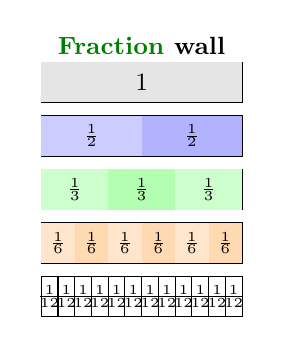
\begin{tikzpicture}[scale=0.85]

\node at (1.5,0.85) {\small\textbf{\ealkey{Fraction} wall}};

\draw (0,0) rectangle (3,0.6);
\fill[gray!20] (0,0) rectangle (3,0.6);
\node at (1.5,0.3) {\small $1$};

\draw (0,-0.8) rectangle (3,-0.2);
\draw (1.5,-0.8) -- (1.5,-0.2);
\fill[blue!20] (0,-0.8) rectangle (1.5,-0.2);
\fill[blue!30] (1.5,-0.8) rectangle (3,-0.2);
\node at (0.75,-0.5) {\tiny $\frac{1}{2}$};
\node at (2.25,-0.5) {\tiny $\frac{1}{2}$};

\draw (0,-1.6) rectangle (3,-1.0);
\foreach \x in {1,2} \draw (\x,-1.6) -- (\x,-1.0);
\fill[green!20] (0,-1.6) rectangle (1,-1.0);
\fill[green!30] (1,-1.6) rectangle (2,-1.0);
\fill[green!20] (2,-1.6) rectangle (3,-1.0);
\node at (0.5,-1.3) {\tiny $\frac{1}{3}$};
\node at (1.5,-1.3) {\tiny $\frac{1}{3}$};
\node at (2.5,-1.3) {\tiny $\frac{1}{3}$};

\draw (0,-2.4) rectangle (3,-1.8);
\foreach \x in {0.5,1,1.5,2,2.5} \draw (\x,-2.4) -- (\x,-1.8);
\foreach \i/\col in {0/orange!20,1/orange!30,2/orange!20,3/orange!30,4/orange!20,5/orange!30} {
  \fill[\col] ({0.5*\i},-2.4) rectangle ({0.5*\i+0.5},-1.8);
  \node at ({0.5*\i+0.25},-2.1) {\tiny $\frac{1}{6}$};
}

\draw (0,-3.2) rectangle (3,-2.6);
\foreach \x in {0.25,0.5,...,2.75} \draw (\x,-3.2) -- (\x,-2.6);
\foreach \i in {0,...,11} {
  \node at ({0.25*\i+0.125},-2.9) {\tiny $\frac{1}{12}$};
}

\end{tikzpicture}
\end{center}

\column{0.8\textwidth}
\small
\begin{enumerate}
\begin{multicols}{2}
\item \ealpara{\ealkeytr{Uprość} całkowicie: $\dfrac{15}{20}$}{Fully \ealkey{simplify}: $\dfrac{15}{20}$}
\ashow{$=\frac{3}{4}$}
\item \ealpara{\ealkeytr{Uprość} całkowicie: $\dfrac{72}{96}$}{Fully \ealkey{simplify}: $\dfrac{72}{96}$}
\ashow{$=\frac{3}{4}$}
\end{multicols}
  \item \ealpara{Użyj \ealkeytr{ściany ułamków}, aby uzupełnić luki:}{Use the \ealkey{fraction} wall to fill in the blanks:}
  \[
    \frac{1}{2} + \frac{\text{{\ashowq{3}}}}{6} = 1 \qquad \frac{\text{{\ashowq{1}}}}{3} + \frac{\text{{\ashowq{4}}}}{6} = 1
  \] 
\begin{multicols}{2}
  \item $2\dfrac{3}{4} + 1\dfrac{2}{3}$ \ashow{$=4\frac{5}{12}$}
  \item $4\dfrac{1}{5} - 1\dfrac{3}{4}$ \ashow{$=2\frac{9}{20}$}
\end{multicols}  
  \item \ealpara{Maya mówi: \textit{``$\frac{1}{2} + \frac{1}{3} = \frac{2}{5}$''}. Wyjaśnij błąd i znajdź poprawną odpowiedź.}{Maya says: \textit{``$\frac{1}{2} + \frac{1}{3} = \frac{2}{5}$''}. Explain the mistake and find the correct answer.}
  \ashow{Dodała również \ealkeytr{mianowniki}; użyj \ealkeytr{wspólnego mianownika}: $\frac36+\frac26=\frac56$.}
  \ashow{She added the \ealkey{denominators} too; use a \ealkey{common denominator}: $\frac36+\frac26=\frac56$.}
  \item \ealpara{Amir zjada $\dfrac{3}{8}$, Beth zjada $\dfrac{1}{4}$, Cal zjada $\dfrac{1}{3}$ pizzy. Jaki \ealkeytr{ułamek} pozostaje?}{Amir eats $\dfrac{3}{8}$, Beth eats $\dfrac{1}{4}$, Cal eats $\dfrac{1}{3}$ of a pizza. What \ealkey{fraction} is left?}
  \ashow{$\frac{1}{24}$}
  \item \ealpara{Uzupełnij luki: $\quad 3\dfrac{1}{4} + \ablank{1\frac{11}{12}} = 5\dfrac{1}{6}$}{Fill in the blanks: $\quad 3\dfrac{1}{4} + \ablank{1\frac{11}{12}} = 5\dfrac{1}{6}$}
  \item \ealpara{Prawda czy fałsz? $\dfrac{a}{b} + \dfrac{a}{c} = \dfrac{2a}{b+c}$. Czy możesz wyjaśnić swoją odpowiedź za pomocą \ealkeytr{dowodu} lub \ealkeytr{kontrprzykładu}?}{True or false? $\dfrac{a}{b} + \dfrac{a}{c} = \dfrac{2a}{b+c}$. Can you explain your answer with a \ealkey{proof}/\ealkey{counterexample}?}
  \ashow{Fałsz; np.\ $a=b=c=1$ daje $2=1$. Poprawnie: $\frac ab+\frac ac=\frac{a(c+b)}{bc}$.}
  \ashow{False; e.g.\ $a=b=c=1$ gives $2=1$. Correct: $\frac ab+\frac ac=\frac{a(c+b)}{bc}$.}
\end{enumerate}

\end{columns}
\end{frame}

\end{document}